%% Manuscript for the Journal of King Saud University - Computer and Information Sciences
%% (Springer Nature). Compile inside the official "Springer Nature LaTeX Template"
%% (v3.1, Overleaf) - it provides sn-jnl.cls and sn-basic.bst. Upload this file,
%% references.bib, tables/ and the PDF figures from ../figures/ into a folder figures/.
%% BLINDED VERSION for double-anonymous review: no author names, affiliations or links that
%% identify the authors. Author details are in title_page.tex.
\documentclass[pdflatex,sn-basic]{sn-jnl}

\usepackage{graphicx}
\usepackage{amsmath,amssymb}
\usepackage{booktabs}
\usepackage{xcolor}
\usepackage{url}

\begin{document}

\title[Explanation-aware incentives against strategic manipulation]{Explanation-Aware
Incentives for Reducing Strategic Manipulation in Multi-Agent AI: A Cross-Domain Evaluation
with Blockchain Provenance}

\author{Anonymous}
\affil{Anonymised for double-anonymous review}

\abstract{When several AI agents decide together, each with its own objective, an agent can
steer the group by voting for the option it privately prefers and attaching a misleading
explanation, and ordinary payoffs neither reward faithful explanations nor penalise false
ones. We propose an explanation-aware incentive: an auditor scores each agent's report for
fidelity to the SHAP attributions of the agent's own model, for evidence supported by the
observed data, and for manipulation, and these scores enter the agent's utility; rewards
accumulate into a reputation that weights votes, and a blockchain records hashes of
decisions, explanations, evidence, rewards and reputation. Under a pre-registered protocol,
five learning agents per domain were evaluated on two real datasets, USAID/PEPFAR
pharmaceutical deliveries (supplier selection) and an energy community with peer-to-peer
trading, with ten paired seeds. The incentive reduced manipulation in both domains
($-69.7\%$ and $-44.4\%$). It improved explanation fidelity and evidence support strongly
where manipulation paid under the baseline (pharmaceutical: $+83.5\%$, $+75.7\%$) and only
negligibly where agents were already largely honest (energy). It did not make collective
decisions more robust to a growing share of agents that always manipulate. The provenance
layer detected all 1{,}000 tampered records without false positives; a hardened variant with
agent signatures and external anchoring refused every forged write and exposed a history
rewritten by its operator, which establishes integrity and authenticity, not truthfulness.
With open LLM agents, a factorial experiment traced the change in behaviour to the wording of
the reward rules rather than to the payoff.}

\keywords{Multi-agent systems, Explainable AI, Mechanism design, Explanation fidelity,
Reputation, Blockchain provenance}

\maketitle

%% ---------------------------------------------------------------------------------------
\section{Introduction}\label{sec:intro}

Decisions that used to be taken by one model are increasingly split among several
specialised AI agents, each responsible for one criterion: cost, reliability, grid
stability, price. Their outputs are combined by a vote or a market, and each agent attaches
an explanation to its contribution so that humans can audit the result. This arrangement
creates an incentive problem that single-model explainability does not face. An agent whose
private objective favours one option can vote for it and attach an explanation that sounds
convincing but does not reflect what its model actually computed, or that cites evidence the
data do not support. Explanation methods are known to be manipulable
\citep{slack2020,dombrowski2019,heo2019}, and plausible but unfaithful rationalisations can be
constructed on purpose \citep{aivodji2019}. In a multi-agent decision, nothing in the usual
payoff, which rewards only the decision, makes a faithful explanation worth more to the agent
than a misleading one.

Mechanism design offers a way to make truthful reporting individually rational, from peer
prediction \citep{miller2005} to the Bayesian truth serum \citep{prelec2004}, and incentive
mechanisms are widely used to steer self-interested learners \citep{zhan2021}. Reputation
systems give persistent weight to agents that behaved well \citep{josang2007,kamvar2003}, and
blockchains can make records of AI decisions tamper-evident \citep{liang2017,nassar2019}.
Recent work combines blockchain with incentives for multi-agent learning \citep{tian2025} or
LLM agent collaboration \citep{kumala2026}, and rewards agents for faithful explanations of a
model \citep{cheng2026}. To our knowledge, however, no study puts explanation fidelity and
evidence support, measured against the agent's own model and the observed data, directly into
the utility of strategic agents that jointly take a decision, and tests the result on real
operational data in more than one domain.

This paper does so. The central question is whether making audited explanation quality part
of each agent's payoff reduces strategic manipulation, and under which conditions it also
improves the explanations themselves. Our contributions are:
\begin{enumerate}
\item An explanation-aware incentive for multi-agent decisions. An auditor with access to each
agent's model scores every report for fidelity, evidence support and manipulation; these
scores enter the agent's utility next to decision quality and contribution; rewards
accumulate into a reputation that weights votes; and a provenance layer records the
artefacts with integrity and, in a hardened variant, authenticity guarantees
(Section~\ref{sec:method}).
\item A pre-registered evaluation on two real datasets with fully specified agents: five
agents per domain with distinct private objectives and feature views, a decision-only
baseline, an ablation without reputation, adversarial and collusion stress tests, tampering
and forgery experiments, cross-domain comparison and sensitivity analysis
(Sections~\ref{sec:setup}--\ref{sec:results}).
\item Evidence on what the mechanism achieves and where it stops. It reduces manipulation in
both domains; it improves explanation quality strongly where manipulation pays under the
baseline and negligibly where agents are already largely honest; it does not protect the
collective decision against agents that ignore the payoff; and with LLM agents the
behavioural change follows the wording of the rules rather than the payoff
(Section~\ref{sec:discussion}).
\end{enumerate}

%% ---------------------------------------------------------------------------------------
\section{Related work}\label{sec:related}

\paragraph{Explanation fidelity.} SHAP attributes a prediction to features with Shapley
values \citep{lundberg2017}, and TreeSHAP computes them exactly for tree ensembles
\citep{lundberg2020}. Whether an explanation reflects the model is its fidelity; evaluation
frameworks and metrics are surveyed by \citet{doshivelez2017} and \citet{zhou2021}, and
\citet{yeh2019} formalise infidelity and sensitivity. \citet{miller2019} argues that
explanations for people must also be selective and contrastive, which is why our agents report
only their top features. We use SHAP of each agent's own model as the reference against which
a reported explanation is scored.

\paragraph{Explanation manipulation.} Post-hoc explainers can be fooled: a model can hide its
reliance on a sensitive feature from LIME and SHAP \citep{slack2020}, saliency maps can be
changed arbitrarily without changing predictions \citep{dombrowski2019,heo2019}, and an
interpretable surrogate can rationalise an unfair model \citep{aivodji2019}. These works study
an adversary who manipulates the explainer; we study agents who misreport their own
explanation, and ask whether incentives can make that unprofitable.

\paragraph{Incentives and reputation.} Peer prediction \citep{miller2005} and the Bayesian truth
serum \citep{prelec2004} reward truthful reports without ground truth; incentive mechanisms for
federated learning reward contributions of self-interested participants \citep{zhan2021}.
Reputation systems aggregate past behaviour into trust \citep{josang2007}, and EigenTrust
does so in peer-to-peer networks \citep{kamvar2003}. Our mechanism has ground truth of a
particular kind available, the agent's own model and the observed data, and rewards agreement
with it.

\paragraph{Blockchain for provenance and trustworthy AI.} ProvChain records data provenance on
a blockchain \citep{liang2017}; \citet{nassar2019} argue for blockchain in explainable and
trustworthy AI. \citet{tian2025} combine blockchain with incentive-compatible multi-agent
reinforcement learning, \citet{kumala2026} propose blockchain-based reputation and incentives
for LLM multi-agent collaboration, and \citet{cheng2026} reward agents for faithful
explanations. None of these puts the fidelity and evidence support of each agent's explanation
into the utility of agents that vote on a shared decision and evaluates it on real data in two
domains.

\paragraph{Application domains.} Supplier selection in pharmaceutical supply chains is a
multi-criteria problem \citep{forghani2018}. Peer-to-peer energy trading and community markets
are reviewed by \citet{tushar2020}, \citet{sousa2019} and \citet{tushar2018}, the latter for
game-theoretic approaches; the Brooklyn Microgrid is a field case \citep{mengelkamp2018}. Our
energy data come from the study of \citet{garciamunoz2025}.

%% ---------------------------------------------------------------------------------------
\section{Proposed framework}\label{sec:method}

Figure~\ref{fig:architecture} shows the pipeline and Figure~\ref{fig:mechanism} the
mechanism. All parameters below were fixed in a protocol frozen before the experiments; later
changes were logged as dated amendments.

\begin{figure*}[t]
\centering
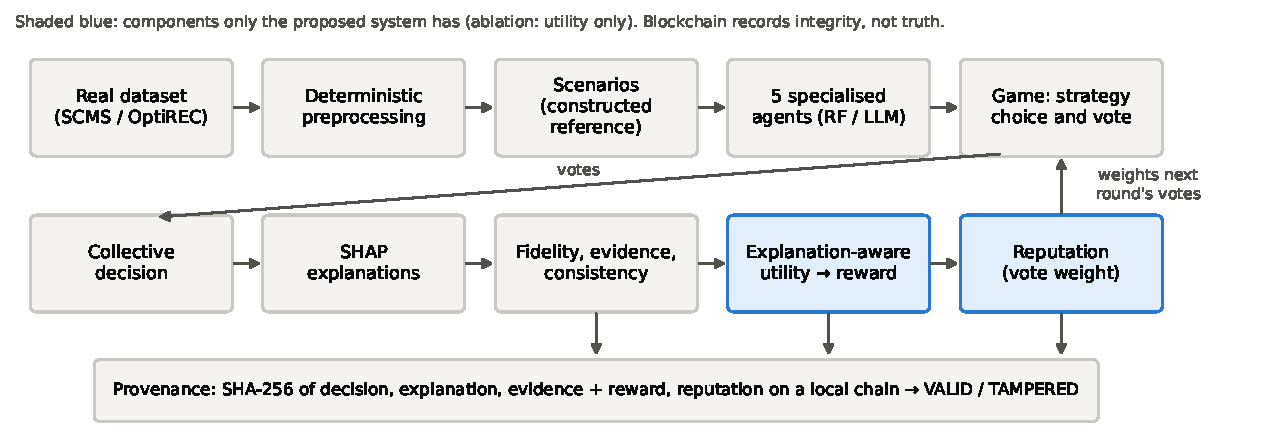
\includegraphics[width=\textwidth]{figures/fig1_architecture.pdf}
\caption{Pipeline. Shaded blue: components that only the proposed system has (the ablation
keeps the explanation-aware utility only). The provenance layer records integrity, not truth}
\label{fig:architecture}
\end{figure*}

\subsection{One round, step by step}\label{sec:round}

The framework separates three things that are easy to conflate: the \emph{agents}, which
predict and report; the \emph{mechanism}, which audits the reports and pays rewards; and the
agents' \emph{learning rule}, which decides how an agent reports next time. The mechanism does
not choose anybody's report; it only changes what each report is worth. A round proceeds as
follows.
\begin{enumerate}
\item \emph{Scenario.} All agents see the same real scenario: a purchase order with three
candidate supplier sites, or one hour of an energy community with a battery decision.
\item \emph{Prediction.} Each agent's own model predicts the reference decision from the
agent's own features; its most probable action is the agent's \emph{model vote}.
\item \emph{Report.} Each agent submits a vote, a confidence, an explanation (two features and
the direction of their effect) and one evidence claim per feature. The report may differ from
what its model says when the agent's private objective favours another action.
\item \emph{Audit.} The auditor compares the explanation with the SHAP attributions of the
agent's model and the evidence claims with the observed data, and computes fidelity,
evidence support and a manipulation score (Section~\ref{sec:metrics}).
\item \emph{Decision, utility and reward.} The votes are combined into the collective
decision; each agent's utility combines its decision quality, fidelity, evidence support,
contribution and manipulation; utilities are rescaled across agents into rewards; rewards
update the reputations that weight the next votes (Section~\ref{sec:incentive}).
\item \emph{Learning.} Each agent receives a payoff that mixes what it gains privately from
the collective decision with its reward, and updates its estimate of how well its chosen
reporting strategy pays (Section~\ref{sec:learning}).
\end{enumerate}

\subsection{Agents, actions and reports}\label{sec:game}

Each domain has five agents $N=\{1,\dots,5\}$ and a finite action set per scenario: three
candidate manufacturing sites in the pharmaceutical case and \{idle, charge, discharge\} for a
community battery in the energy case. Agent $i$ has a private objective $u_i(a)$, a
closed-form function of real or derived variables, normalised to $\tilde u_i(a)\in[0,1]$ over
the actions of the scenario; its privately preferred action maximises $\tilde u_i$. Each agent
also has a model, a random forest \citep{breiman2001} with 100 trees of depth 6 trained on its
own feature view to predict the reference decision. The private objective and the model can
disagree, and that disagreement is what creates an incentive to misreport. The objectives and
features of all ten agents are listed in Table~\ref{tab:agents} (Section~\ref{sec:setup}).

A report is a vote, a confidence, an explanation of $k=2$ (feature, sign) pairs, and one
evidence claim per explained feature stating its level (low, mid or high by training-set
terciles). The strategy set has five elements. \emph{Honest} reports the model vote, the
model's probability, the top-$k$ SHAP features with their true signs and true levels.
\emph{Strategic} switches to its privately preferred action when that gains at least 0.25 in
$\tilde u_i$ and then inflates its confidence by 0.3, but explains truthfully.
\emph{Misattributing} and \emph{overclaiming} vote like strategic but replace one explained
feature by an unimportant one with a flipped sign, or one evidence level by a false one.
\emph{Manipulative} always votes for its preferred action with confidence 1 and reports the
$k$ least important features with flipped signs and false levels. These strategies change
reports only; the observations are never altered. The collective decision is a weighted
confidence vote, $\arg\max_a \sum_i w_i\, c_i\, \mathbb{1}[v_i=a]$, with $w_i=1$ in the
baseline and ablation and $w_i=\mathrm{Rep}_i$ in the proposed system.

\subsection{Auditing explanations}\label{sec:metrics}

The auditor has white-box access to each agent's model and computes exact TreeSHAP
attributions $\phi$ for the voted action \citep{lundberg2020}. Three per-round scores follow.

\emph{Fidelity} is the share of the true top-$k$ attribution mass that the agent reported with
the correct sign,
\begin{equation}
F_i=\frac{\sum_{f\in \mathcal{E}_i,\ \mathrm{sign}\ \mathrm{correct}}|\phi_f|}
{\sum_{f\in \mathrm{top}\text{-}k(|\phi|)}|\phi_f|}\in[0,1],
\end{equation}
with $F_i=0$ for an empty explanation and $F_i=1$ when all attributions are zero.
\emph{Evidence support} $E_i$ is the share of the agent's claims whose stated level matches
the observed value. \emph{Manipulation} $M_i$ is the mean of five audited components: false
attribution $1-F_i$; confidence inflation $\max(0, c_i-p_i)$, where $p_i$ is the model's
probability of the vote; unsupported evidence $1-E_i$; strategic voting
$\mathbb{1}[v_i\neq \text{model vote}]$; and collusion, flagged when an agent deviates from
its model and another deviating agent casts the same vote. $M_i$ is computed from reports and
the audit only, never from knowledge of the strategy played. As secondary outcomes we report
explanation consistency (Jaccard similarity of explanations across the five most similar
scenarios), collective accuracy and manipulation success (the collective action is wrong and
equals the vote of an agent that deviated from its model).

\subsection{Explanation-aware utility, reward and reputation}\label{sec:incentive}

\begin{figure*}[t]
\centering
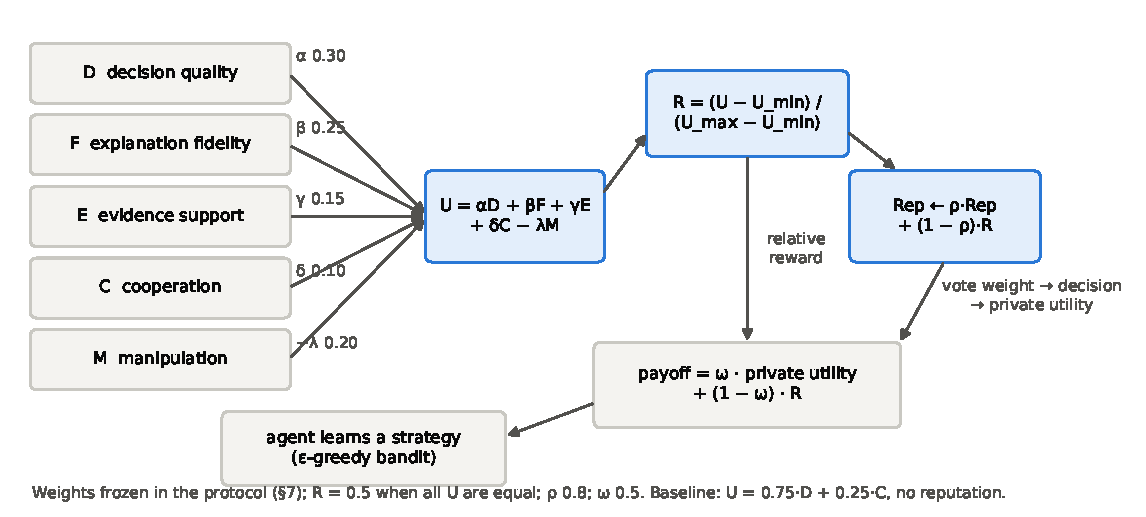
\includegraphics[width=0.92\textwidth]{figures/fig2_mechanism.pdf}
\caption{The explanation-aware incentive. The utility combines five audited components; the
reward is the utility rescaled across agents; reputation accumulates rewards and weights the
next votes; the agent's payoff mixes its private utility of the collective action with the
reward}
\label{fig:mechanism}
\end{figure*}

The utility of agent $i$ in a round is
\begin{equation}
U_i=\alpha D_i+\beta F_i+\gamma E_i+\delta C_i-\lambda M_i,\label{eq:utility}
\end{equation}
with $D_i=\mathbb{1}[v_i$ equals the reference decision$]$ and $C_i\in\{0,0.5,1\}$ the
agent's pivotal contribution (1 if removing its vote would turn a correct collective
decision into a wrong one, 0 for the reverse, 0.5 otherwise). The weights $\alpha=0.30$,
$\beta=0.25$, $\gamma=0.15$, $\delta=0.10$ and $\lambda=0.20$ were set a priori. The
baseline uses $U_i=0.75D_i+0.25C_i$, the same ratio of decision to contribution with no
explanation terms: under it, an explanation earns or costs nothing. The reward rescales
utilities across the agents of the round, $R_i=(U_i-U_{\min})/(U_{\max}-U_{\min})$, with
$R_i=0.5$ when all utilities are equal, so an agent is paid for doing better than the others
in the same round. Reputation starts at 0.5 and is updated as
$\mathrm{Rep}_i\leftarrow\rho\,\mathrm{Rep}_i+(1-\rho)R_i$ with $\rho=0.8$, an effective
memory of about five rounds. The mechanism therefore acts through two channels: a false
report lowers the agent's reward in the round in which it is made and, through reputation,
the weight of its vote in later rounds.

\begin{table*}[t]
\caption{Worked example: the lead-time agent in one round of the pharmaceutical proposed run (seed 0, round 354). The same round is scored with the agent's honest and manipulative report, the other agents' reports fixed}\label{tab:example}
\footnotesize
\begin{tabular}{@{}p{0.24\textwidth}p{0.36\textwidth}p{0.36\textwidth}@{}}
\toprule
 & Honest report & Manipulative report \\
\midrule
Vote, confidence & site 2, 0.38 & site 1, 1.00 \\
Explanation & lead-time records raises; lead time (relative) raises & lead-time records raises; median lead time lowers \\
Evidence claims & lead-time records high (observed high); lead time (relative) high (observed high) & lead-time records high (observed low); median lead time high (observed low) \\
Fidelity $F$ & 1.00 & 0.00 \\
Evidence $E$ & 1.00 & 0.00 \\
Manipulation $M$ & 0.00 & 0.75 \\
Decision $D$ & 0.00 & 0.00 \\
Contribution $C$ (proposed) & 0.50 & 0.50 \\
Utility $U$ (proposed) & $+0.450$ & $-0.100$ \\
Reward $R$ (proposed) & 0.296 & 0.000 \\
Collective decision (proposed) & site 3 & site 3 \\
Payoff $\pi$ (proposed) & 0.388 & 0.240 \\
Contribution $C$ (baseline) & 0.00 & 0.00 \\
Utility $U$ (baseline) & $+0.000$ & $+0.000$ \\
Reward $R$ (baseline) & 0.000 & 0.000 \\
Collective decision (baseline) & site 2 & site 1 \\
Payoff $\pi$ (baseline) & 0.000 & 0.500 \\
\bottomrule
\end{tabular}
\footnotetext{Model vote site 2 (probabilities 0.26, 0.38, 0.36); privately preferred site 1 (normalised private utility 1.00, 0.00, 0.48); reference site 3; reputation 0.217. Payoff $\pi=\omega\tilde u_i(a^\ast)+(1-\omega)R$ with $\omega=0.5$. Baseline rows: the same reports paid by the decision-only utility with equal votes.}
\end{table*}


\paragraph{Worked example.} Table~\ref{tab:example} shows one real round of the
pharmaceutical proposed run, chosen by a fixed rule (the first evaluation round in which a
learning agent played manipulative while its preferred site differed from both its model vote
and the reference). The lead-time agent's model favours site~2, its private objective favours
site~1, and the reference is site~3. An honest report explains the model correctly ($F=E=1$,
$M=0$) and earns a reward of 0.296. The manipulative report votes for site~1 with confidence
1 and attaches an explanation and evidence that the audit rejects ($F=E=0$, $M=0.75$); its
utility becomes negative and its reward 0. Because the agent's reputation is low (0.217), its
vote does not change the collective decision, so manipulation gains nothing privately and the
honest report pays more (0.388 against 0.240). Paid by the decision-only baseline with equal
votes, the same manipulative report would have moved the collective decision to the agent's
preferred site and paid 0.500, against 0.000 for honesty. The round is an illustration; over
all 1{,}500 agent-rounds of the evaluation window, replacing an agent's honest report by a
manipulative one (the others' reports as played) paid more in 40.3\% of cases under the
baseline payoff and in 18.5\% under the proposed one, with mean payoff differences of
$+0.150$ and $-0.164$.

\subsection{How agents learn}\label{sec:learning}

Agents choose a strategy each round with a stateless $\varepsilon$-greedy bandit
($\varepsilon=0.1$, learning rate 0.1) on the payoff
\begin{equation}
\pi_i=\omega\,\tilde u_i(a^{\ast})+(1-\omega)\,R_i,\qquad \omega=0.5,\label{eq:payoff}
\end{equation}
where $a^{\ast}$ is the collective action. The first term is what an agent gains privately by
steering the decision; $\omega$ sets how much that matters relative to the mechanism's reward.
The bandit is not part of the mechanism: it is a simple model of self-interested agents that
repeat what has paid. The mechanism succeeds if, under it, the strategies that pay are the
truthful ones. We do not claim that the learning dynamics reach a Nash equilibrium; instead
we report, for the all-honest profile, the payoff of every unilateral deviation.

\subsection{Provenance layer}\label{sec:provenance}

We distinguish three properties a record of an agent's output can have. \emph{Integrity}: a
change after recording is detectable. \emph{Authenticity}: the record was produced and signed
by the registered agent. \emph{Truthfulness}: the record describes what the agent's model
actually computed. A blockchain can provide the first two; only the audit of
Section~\ref{sec:metrics} addresses the third.

For every agent and round, the provenance layer stores on chain the SHA-256 hashes of the
canonically serialised decision, explanation and evidence, together with the reward and
reputation scaled to integers ($\times10^{6}$) and a block timestamp; the artefacts
themselves stay off chain. A Solidity contract makes records append-only and writable only
by the deploying account. Verification recomputes the hashes from the off-chain store and
reports each record as valid, tampered or missing. This basic design provides integrity, but
it trusts the operator who writes the records. A hardened variant, added after the
main provenance results were known, removes part of that trust with three additions. First,
\emph{model registration}: each agent is bound once to a signing key and to the hash of its
model identity (model, digest, decoding settings and the agent's objective). Second,
\emph{agent signatures}: the contract accepts a record only if the agent's registered key
signed its identifier, artefact hashes and model hash for this chain and contract, so the
operator cannot forge or replay an agent's output. Third, \emph{anchoring}: Merkle roots
\citep{laurie2013} of the registrations and of every 1{,}000 records are written to
a second chain that the operator is assumed unable to rewrite, so a rebuilt history no longer
matches the anchors. Rewards and reputations are computed by the mechanism and are therefore
covered by the anchors but not by the agents' signatures. The hardened variant adds
authenticity for the agent-produced artefacts; neither variant establishes truthfulness.

\subsection{LLM agents}\label{sec:llm}

As an extension, we replaced the five classical agents with an open LLM, Qwen2.5-7B
\citep{qwen2024}, served locally with Ollama at temperature 0. Each LLM agent receives the
scenario, the output of its model (prediction and SHAP attributions) and the reward rules, and
must write its own report in the fixed format above, which is audited exactly as before.

\subsection{Use of generative AI}\label{sec:ai}

The experiment code, analysis scripts and a first draft of this manuscript were produced with
an AI coding assistant (Anthropic's Claude, used through Claude Code) under the author's
direction. All reported numbers are generated by that code from the saved results; tables and
figures are produced by scripts from the result files; every reference was retrieved from
Crossref, DataCite or arXiv by its identifier. The author reviewed the design, the protocol
amendments and the text. Qwen2.5-7B served as the experimental subject in
Section~\ref{sec:llm}, not as a writing aid.

%% ---------------------------------------------------------------------------------------
\section{Experimental design}\label{sec:setup}

\begin{table*}[t]
\caption{Case studies, scenarios and preprocessing}\label{tab:data}
\footnotesize
\begin{tabular}{@{}lp{5.2cm}p{5.2cm}@{}}
\toprule
 & Pharmaceutical & Energy \\
\midrule
Source & USAID/PEPFAR SCMS delivery history \citep{scmsdata2015} & OptiREC energy community \citep{optirecdata2025} \\
Scenario & one purchase order, three candidate sites & one hour of the community \\
Scenarios & 1,648 (31 products, 49 sites) & 8,760 \\
Train / val / test & 824 / 165 / 659 (by order date) & 5,400 / 1,680 / 1,680 (week blocks) \\
Agents & cost, reliability, lead time, logistics, continuity & producer, consumer, market, grid, storage \\
Reference decision & equal-weight multi-criteria score (constructed) & daily perfect-foresight LP (constructed) \\
Simulated inputs & candidate set & battery: C-rate 0.5, efficiency 0.9 \\
Derived variables & 27 & 12 \\
\bottomrule
\end{tabular}
\end{table*}


Both case studies use real operational data. Agents, scenarios and reference decisions are
built from the data by deterministic, documented rules; every derived variable is a function
of recorded columns, and nothing in the observations is changed by the strategies or attacks.
Table~\ref{tab:data} summarises the two datasets and Table~\ref{tab:agents} the ten agents.

\begin{table*}[t]
\caption{The five agents of each case study: private objective and the features its model sees}\label{tab:agents}
\footnotesize
\begin{tabular}{@{}lp{4.6cm}p{7.2cm}@{}}
\toprule
Agent & Prefers the action with & Features \\
\midrule
\multicolumn{3}{@{}l}{\emph{Pharmaceutical supplier selection (action: one of three candidate sites)}} \\
cost & lowest expected unit price & expected unit price, price relative to candidates, last price (relative), price variability, order size \\
reliability & highest past on-time delivery rate & on-time rate, on-time rate (relative), mean days late, past deliveries, late share of last five \\
lead time & shortest past median lead time & median lead time, lead time (relative), lead-time spread, lead-time records, requested lead time \\
logistics & lowest past freight cost per kg & freight per kg, freight (relative), share shipped by air, share with freight included, past deliveries to the country \\
continuity & most past deliveries of the product & past deliveries of the product, share of the product among candidates, days since last delivery, countries served, units of the product supplied \\
\midrule
\multicolumn{3}{@{}l}{\emph{Peer-to-peer energy (action: charge, idle or discharge the community battery)}} \\
producer & export when the feed-in price is above its daily median & PV availability, temperature, hour of day, feed-in price, feed-in price rank in the day \\
consumer & lowest cost of grid imports & community load, thermal demand, temperature, flexibility availability, import price, hour of day \\
market & charge when the import price is below its daily median, discharge when above & import price, feed-in price, gas price, import price rank in the day, import minus feed-in price \\
grid & smallest absolute exchange with the grid & net demand (load $-$ PV), community load, PV availability, hour of day \\
storage & charge on community surplus, otherwise stay idle & net demand (load $-$ PV), EVs at home, hour of day, import price rank in the day, PV availability \\
\bottomrule
\end{tabular}
\footnotetext{Each agent's private objective is normalised to $[0,1]$ over the actions of a scenario; its privately preferred action is the maximiser. Each agent has its own random forest (100 trees, depth 6) trained on its own features to predict the reference decision; its argmax is the agent's model vote, and SHAP of this model is the reference for its explanation. Pharmaceutical features describe the candidate site and are computed only from deliveries completed before the order date; feature views do not overlap.}
\end{table*}


\subsection{Pharmaceutical supplier selection}\label{sec:pharma}

\paragraph{Data.} The USAID/PEPFAR Supply Chain Management System delivery history
\citep{scmsdata2015} contains 10{,}324 shipment line items of antiretroviral drugs and HIV
test kits delivered between 2006 and 2015. A line records, among other fields, the purchase
order, product, manufacturing site, destination country, shipment mode, scheduled and actual
delivery dates, pack price, units, weight and freight cost. We use only the 4{,}920
direct-from-supplier lines, because on warehouse lines the delivery performance is not the
manufacturer's. A supplier is a manufacturing site; a product is a molecule or test type
with its dosage and form.

\paragraph{Scenarios.} A scenario is one purchase order for one product with three candidate
sites: the three sites that most recently delivered that product before the order date, among
sites with a recorded price. The data contain no competing offers, so the candidate set is an
experimental construction; the site actually used is among the three in 83\% of scenarios.
Everything known about a candidate is computed only from deliveries completed before the
order date, which prevents leakage from the order's own outcome: expected unit price (median
of its five most recent prices), on-time delivery rate, median lead time, freight cost per
kilogram, past deliveries of the product and related variables (27 derived variables in all).
A site without lead-time or freight history receives the all-sites median (2.7\% of candidate
rows for lead time). The result is 1{,}648 scenarios over 31 products and 49 sites, split by
order date into 824 training, 165 validation and 659 test scenarios.

\paragraph{Reference decision.} Each of five criteria (cost, delivery reliability, lead time,
freight cost per kilogram, supply continuity) is min--max normalised over the three
candidates, and the reference is the candidate with the highest equal-weight sum, in the
spirit of multi-criteria supplier selection \citep{forghani2018}. Equal weights are used
because the source gives none. This is a constructed reference, not a record of good
decisions: where the site actually used is a candidate, the reference picks it in 35\% of
scenarios, close to chance (33\%). Dropping one criterion leaves the reference unchanged in
68--74\% of scenarios and doubling one in 72--82\%.

\paragraph{Agents.} Each agent represents one criterion and prefers the candidate that is
best on it (Table~\ref{tab:agents}); its model sees five features of that criterion only. Each
agent's preferred site coincides with the reference in 46--52\% of scenarios, so every agent
often has a private reason to vote against the reference. This conflict is what makes
manipulation profitable under a decision-only payoff.

\subsection{Peer-to-peer energy}\label{sec:energy}

\paragraph{Data.} The OptiREC dataset \citep{optirecdata2025,garciamunoz2025} contains one
year of hourly operational data of a 55-user energy community under peer-to-peer trading and
flexibility markets: per-user load profiles and generation capacities, PV availability, import and
feed-in prices, gas price, temperature, thermal demand, flexibility availability, electric
vehicle presence and battery capacity. It has no missing values; no outlier was removed.
Derived variables (12) are deterministic functions of the recorded columns, for example
community load, PV output, net demand (load minus PV), and the rank of the hour's price within
its day.

\paragraph{Scenarios and reference decision.} A scenario is one hour (8{,}760 in all), and the
decision is the action of an aggregate community battery: charge, idle or discharge. The data
record no storage dispatch, so the reference is the solution of a daily perfect-foresight
linear programme that minimises import cost minus feed-in revenue subject to the battery's
energy balance. The battery capacity is taken from the data; its C-rate (0.5), round-trip
efficiency (0.9), state-of-charge window (10--90\%) and daily start and end state (50\%) are
simulated assumptions, because the dataset does not provide them. The reference is therefore
constructed as well, and decision accuracy means agreement with this programme, not with
observed behaviour. Splits use whole weeks in five-week cycles (three for training, one for
validation, one for testing; 5{,}400, 1{,}680 and 1{,}680 hours), which prevents temporal
leakage.

\paragraph{Agents.} The producer, consumer, market, grid and storage agents represent the
perspectives of a P2P community (Table~\ref{tab:agents}). Their objectives are driven by
prices and surplus, as is the reference programme, so they conflict with the reference less
often than the pharmaceutical criteria do; the results in Section~\ref{sec:main} show what
this implies.

\subsection{Systems compared}\label{sec:systems}

Three systems are run on identical scenarios and seeds (paired design): the \emph{baseline}
(game and explanations, decision-only utility, equal votes), the \emph{ablation}
(explanation-aware utility, equal votes) and the \emph{proposed} system (explanation-aware
utility and reputation-weighted votes). Each system is run with seeds 0--9: 600 rounds with
evaluation on the last 300 in pharma, 1{,}000 rounds and the last 500 in energy.

\subsection{Hypotheses and statistical analysis}\label{sec:hypotheses}

The protocol pre-registered six hypotheses, each comparing the proposed system with the
baseline:
\begin{itemize}
\item[H1] the proposed system improves explanation fidelity;
\item[H2] it improves evidence support;
\item[H3] it reduces manipulation;
\item[H4] it is more robust to an increasing share of malicious agents;
\item[H5] the provenance layer detects modification of recorded artefacts;
\item[H6] H1--H3 give the same verdict in both domains.
\end{itemize}
H1--H3 form the confirmatory family, tested per domain with a paired $t$-test or, when
Shapiro--Wilk rejects normality, a Wilcoxon signed-rank test, with Holm correction
\citep{holm1979} across the three. The pre-registered decision rule calls an outcome
\emph{improved} if the Holm-adjusted $p<0.05$ in the hypothesised direction and the relative
change $(\text{proposed}-\text{baseline})/|\text{baseline}|$ is at least 5\%, \emph{worse} if
significant in the opposite direction, and \emph{negligible} otherwise. The 5\% threshold
separates practical from merely statistical significance: a significant change smaller than
5\% is reported as negligible. H4 is tested as a stress test: malicious shares of 0--40\%
(malicious agents always play manipulative, whatever the payoff), comparing the mean accuracy
degradation over 10--40\% between systems with a paired test; collusion uses two colluding
agents and three honest ones. H5 is descriptive. H6 holds for an outcome when both domains
give the same verdict; domains are never pooled. The comparison of the proposed system with
the ablation, which isolates the contribution of reputation, is a secondary analysis. The
sensitivity analysis varies one parameter at a time: $\beta\in\{0,0.1,0.25,0.4\}$,
$\rho\in\{0.5,0.8,0.95\}$ and $\omega\in\{0.25,0.5,0.75\}$. The LLM agents (Section~\ref{sec:llm})
answer a separate question, whether such agents respond to the payoff at all; they were run
for 200 rounds with seeds 0--4 and are reported apart from the confirmatory family.

%% ---------------------------------------------------------------------------------------
\section{Results}\label{sec:results}

\subsection{Explanation quality and manipulation}\label{sec:main}

\begin{table*}[t]
\caption{Baseline vs proposed, classical agents ($n=10$ paired seeds; mean $\pm$ SD). Verdicts: pre-registered rule (Holm $p<0.05$ in the hypothesised direction and $|\mathrm{rel.}|\geq 5\%$)}\label{tab:main}
\footnotesize
\begin{tabular}{@{}llllllll@{}}
\toprule
Domain & Metric & Baseline & Proposed & $\Delta$ [95\% CI] & Rel. & $p$ (Holm) & Verdict \\
\midrule
pharma & Fidelity $F$ & 0.510 $\pm$ 0.077 & 0.936 $\pm$ 0.020 & +0.426 [+0.370, +0.482] & +83.5\% & $<0.0001$ & improved \\
 & Evidence support $E$ & 0.522 $\pm$ 0.070 & 0.917 $\pm$ 0.023 & +0.395 [+0.345, +0.444] & +75.7\% & $<0.0001$ & improved \\
 & Manipulation $M$ & 0.392 $\pm$ 0.038 & 0.119 $\pm$ 0.015 & -0.273 [-0.302, -0.243] & -69.7\% & $<0.0001$ & improved \\
 & Collective accuracy & 0.578 $\pm$ 0.045 & 0.606 $\pm$ 0.033 & +0.029 [-0.018, +0.076] & +5.0\% & 0.2021$^{a}$ & -- \\
 & Manipulation success & 0.398 $\pm$ 0.057 & 0.263 $\pm$ 0.032 & -0.135 [-0.185, -0.085] & -33.9\% & 0.0002$^{a}$ & -- \\
\midrule
energy & Fidelity $F$ & 0.936 $\pm$ 0.024 & 0.970 $\pm$ 0.004 & +0.034 [+0.021, +0.050] & +3.6\% & 0.0039 & negligible \\
 & Evidence support $E$ & 0.926 $\pm$ 0.031 & 0.966 $\pm$ 0.004 & +0.040 [+0.017, +0.063] & +4.3\% & 0.0039 & negligible \\
 & Manipulation $M$ & 0.066 $\pm$ 0.017 & 0.036 $\pm$ 0.005 & -0.029 [-0.043, -0.016] & -44.4\% & 0.0026 & improved \\
 & Collective accuracy & 0.744 $\pm$ 0.019 & 0.754 $\pm$ 0.013 & +0.009 [-0.000, +0.019] & +1.2\% & 0.0541$^{a}$ & -- \\
 & Manipulation success & 0.050 $\pm$ 0.017 & 0.025 $\pm$ 0.012 & -0.025 [-0.037, -0.012] & -49.4\% & 0.0015$^{a}$ & -- \\
\bottomrule
\end{tabular}
\footnotetext{$^{a}$Secondary outcome, unadjusted $p$, no verdict.}
\end{table*}


\begin{figure*}[t]
\centering
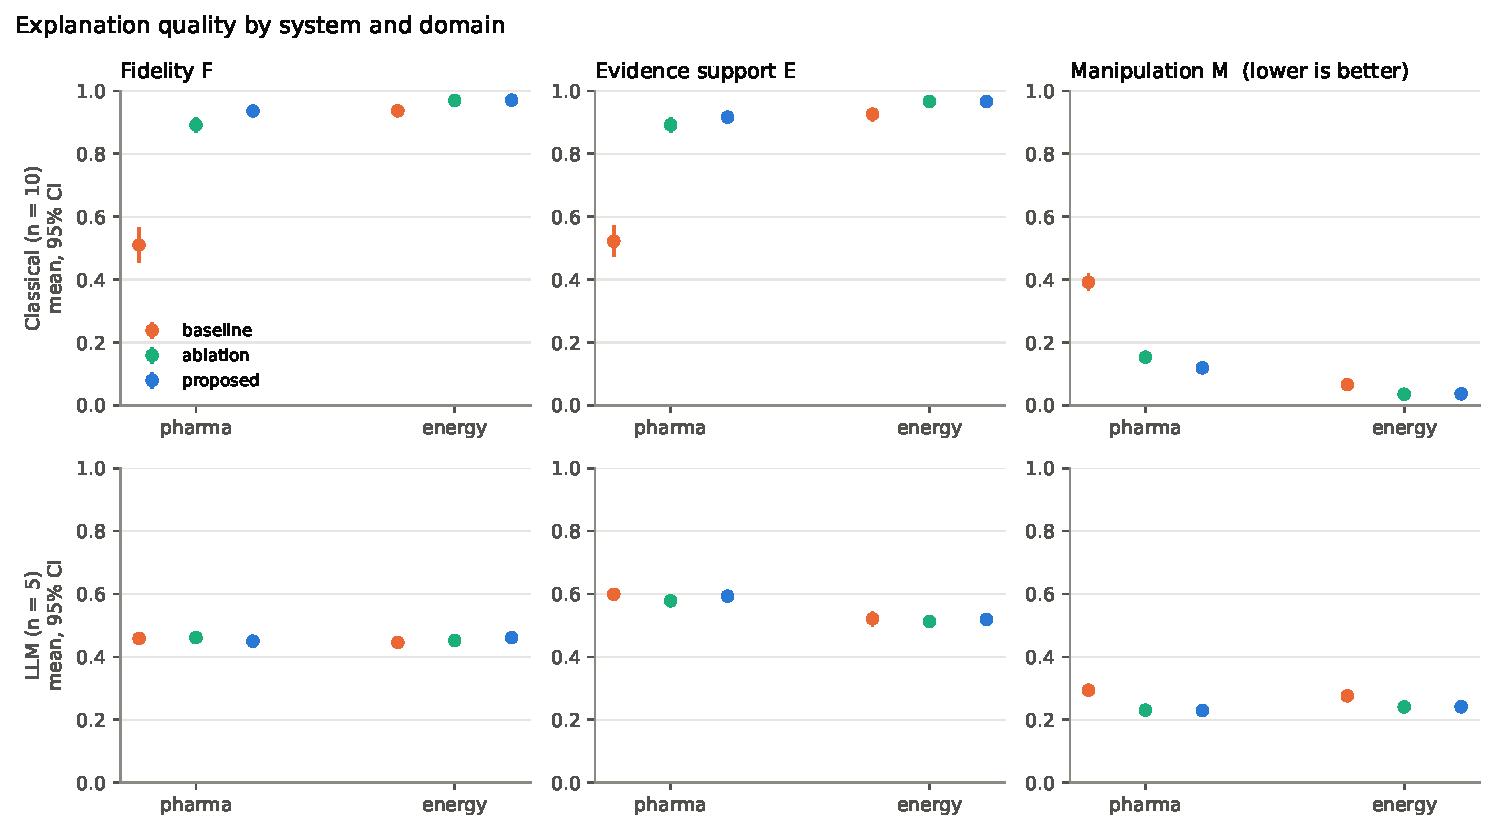
\includegraphics[width=\textwidth]{figures/fig3_explanation_quality.pdf}
\caption{Fidelity, evidence support and manipulation by system and domain, for classical
(top) and LLM agents (bottom); points are means, bars 95\% confidence intervals}
\label{fig:quality}
\end{figure*}

Table~\ref{tab:main} and Figure~\ref{fig:quality} show the main comparison. In the
pharmaceutical case the incentive raised fidelity from 0.510 to 0.936 ($+83.5\%$) and
evidence support from 0.522 to 0.917 ($+75.7\%$), and cut manipulation from 0.392 to 0.119
($-69.7\%$); all three are improved under the decision rule (Holm $p<0.0001$). In energy,
manipulation fell from 0.066 to 0.036 ($-44.4\%$, improved), while fidelity ($+3.6\%$) and
evidence support ($+4.3\%$) rose significantly but below the 5\% threshold, so both are
negligible. The energy baseline already reached $F=0.936$ and $E=0.926$, leaving little room
to improve; we report this as context and do not change the verdict. Collective accuracy did
not change detectably in either domain, while manipulation success fell by a third in pharma
and by half in energy (secondary outcomes). Explanation consistency rose by 28.6\% and 8.6\%.

Why the two domains differ is visible in what the agents learned. Under the baseline, the
pharmaceutical agents played honest in only 9.5\% of evaluation rounds and manipulative in
41.1\%; under the proposed system, 41.4\% and 3.0\%. The energy agents were honest in 77.5\% of
rounds already under the baseline (87.6\% under the proposed system), because their
objectives rarely pay them to steer the battery away from the reference. Where there is
little manipulation to remove, there is little explanation quality to gain. The relative
changes should be read with this in mind: a relative change measures improvement over the
baseline's level, so the same mechanism produces a large relative gain where the baseline
is poor and a small one where it is already near its ceiling.

The unilateral-deviation analysis qualifies these results. In energy, honesty is the best
response for all five agents in every system, so the baseline is already close to honest. In
the pharmaceutical case, honesty is the best response for no agent under the baseline and for
two of five under the proposed system; the other three gain most from strategic voting with a
truthful explanation. The incentive therefore removes the profit of false explanations
without making the all-honest profile an equilibrium.

\subsection{Ablation: incentive versus reputation}\label{sec:ablation}

\begin{table}[t]
\caption{Incentive ablation (incentive without reputation) vs baseline, and the descriptive increment of reputation (proposed $-$ ablation)}\label{tab:ablation}
\footnotesize
\begin{tabular}{@{}llllll@{}}
\toprule
Domain & Metric & Rel. & $p$ (Holm) & Verdict & Reputation increment \\
\midrule
pharma & Fidelity $F$ & +74.9\% & $<0.0001$ & improved & +0.044 \\
 & Evidence support $E$ & +70.9\% & $<0.0001$ & improved & +0.025 \\
 & Manipulation $M$ & -61.0\% & $<0.0001$ & improved & -0.034 \\
energy & Fidelity $F$ & +3.5\% & 0.0037 & negligible & +0.001 \\
 & Evidence support $E$ & +4.4\% & 0.0037 & negligible & -0.001 \\
 & Manipulation $M$ & -46.2\% & 0.0013 & improved & +0.001 \\
\bottomrule
\end{tabular}
\end{table}


\begin{figure*}[t]
\centering
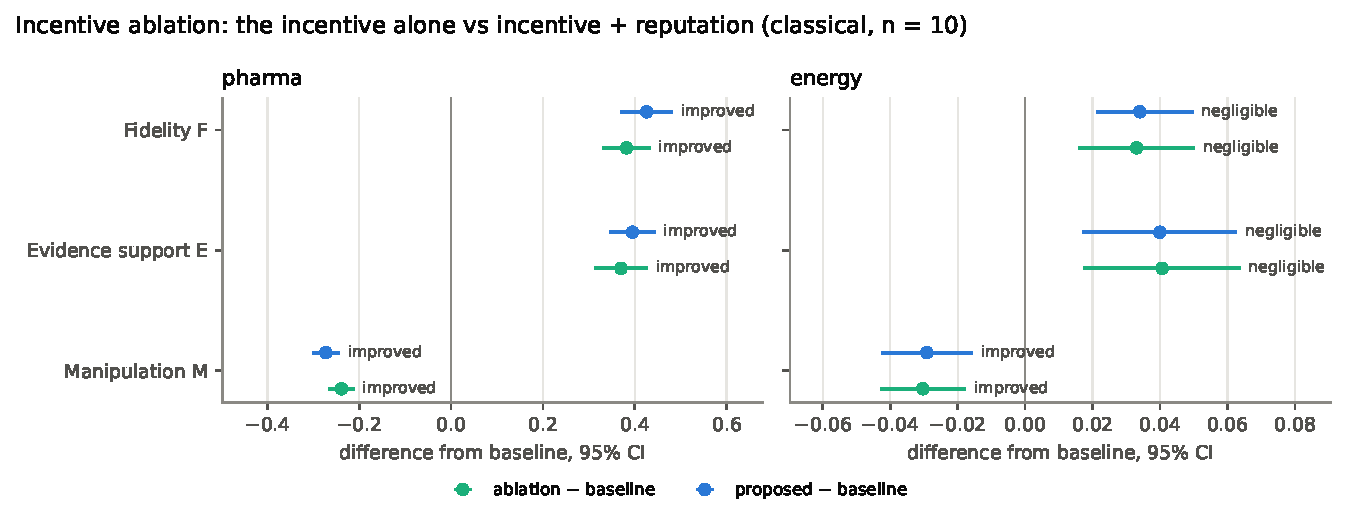
\includegraphics[width=\textwidth]{figures/fig6_ablation.pdf}
\caption{Difference from the baseline for the ablation (incentive only) and the proposed
system (incentive and reputation), with 95\% confidence intervals and verdicts}
\label{fig:ablation}
\end{figure*}

The explanation-aware utility alone produces most of the effect (Table~\ref{tab:ablation},
Figure~\ref{fig:ablation}): the ablation reaches the same verdicts as the proposed system in
both domains, with relative changes in pharma of $+74.9\%$ (fidelity), $+70.9\%$ (evidence)
and $-61.0\%$ (manipulation). Reputation-weighted voting adds a small further gain in pharma
(fidelity $+0.044$, manipulation $-0.034$) and none in energy; this comparison is descriptive.

\subsection{Adversarial stress test: a boundary of the mechanism (H4)}\label{sec:robust}

\begin{table*}[t]
\caption{Robustness. H4: mean accuracy degradation over 10--40\% malicious agents, proposed $-$ baseline (negative = proposed degrades less; paired $t$-test). Collusion: change in manipulation success (baseline / proposed) and in the colluders' reward under the proposed system when two agents collude (unadjusted)}\label{tab:robust}
\footnotesize
\begin{tabular}{@{}llllll@{}}
\toprule
Domain & H4 $\Delta$ [95\% CI] & $p$ & Verdict & Collusion: manip. success & Colluders' reward \\
\midrule
pharma & +0.039 [-0.009, +0.087] & 0.1021 & not supported & +0.380 / +0.126 & -0.458 \\
energy & -0.020 [-0.043, +0.002] & 0.0684 & not supported & +0.155 / +0.047 & -0.501 \\
\bottomrule
\end{tabular}
\end{table*}


\begin{figure*}[t]
\centering
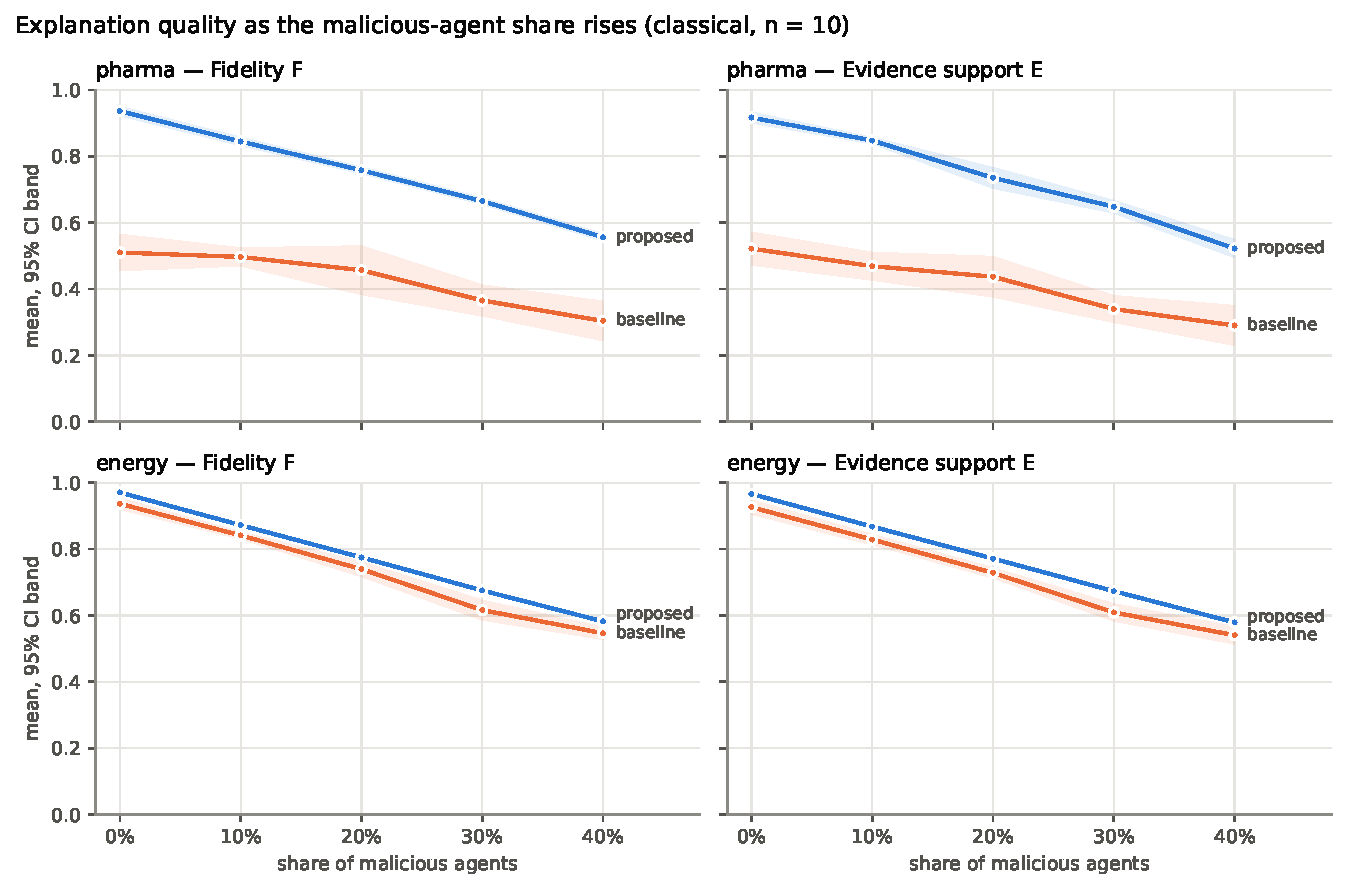
\includegraphics[width=\textwidth]{figures/fig4_quality_vs_malicious.pdf}
\caption{Fidelity and evidence support as the share of malicious agents rises (means and 95\%
confidence bands)}
\label{fig:malicious_quality}
\end{figure*}

\begin{figure*}[t]
\centering
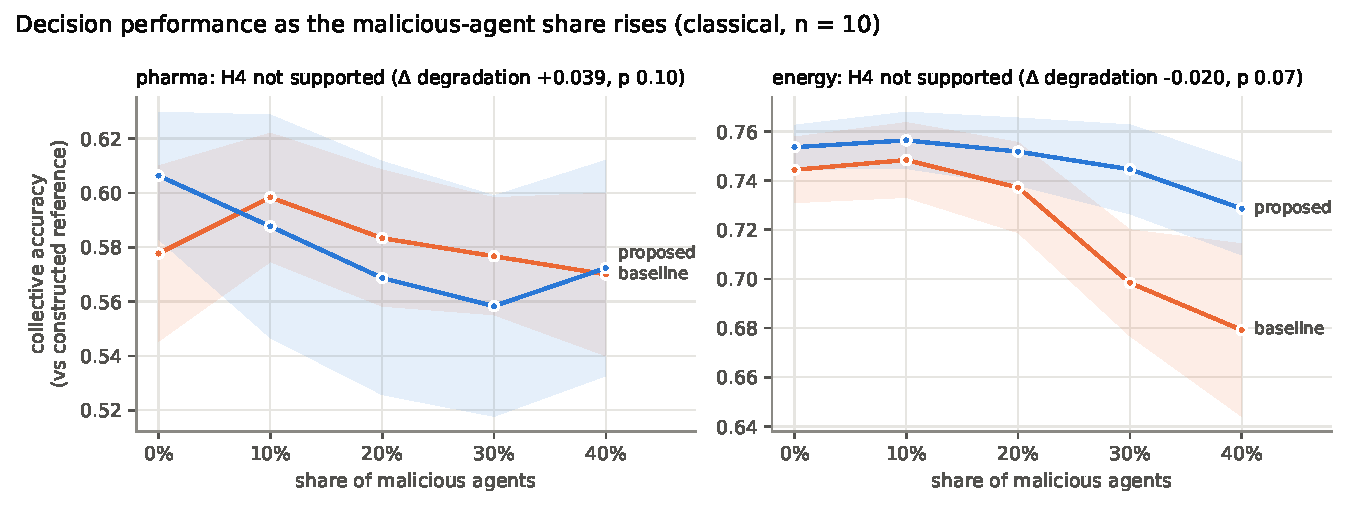
\includegraphics[width=\textwidth]{figures/fig5_decision_vs_malicious.pdf}
\caption{Collective accuracy as the share of malicious agents rises}
\label{fig:malicious_accuracy}
\end{figure*}

This experiment asks a different question from H1--H3. There, agents choose their reports
and the mechanism changes what pays; here, a growing share of agents manipulates every round
regardless of the payoff. H4 is not supported (Table~\ref{tab:robust}). The proposed system's
accuracy did not degrade
less than the baseline's as malicious agents rose from 10 to 40\%: the mean difference in
degradation was $+0.039$ ($p=0.10$) in pharma and $-0.020$ ($p=0.068$) in energy
(Figure~\ref{fig:malicious_accuracy}). The proposed system keeps clearly higher fidelity and
evidence support than the baseline at every malicious share, but both fall roughly linearly
as the share grows (Figure~\ref{fig:malicious_quality}): the audit scores what malicious agents
report, and the mechanism cannot make them report differently. Under collusion, the mechanism
takes the reward away from the colluders ($-0.458$ in pharma, $-0.501$ in energy) and the
honest agents' payoff rises; collusion still raises manipulation success, but by less than
under the baseline ($+0.126$ against $+0.380$ in pharma; $+0.047$ against $+0.155$ in energy).

\subsection{Provenance: integrity and authenticity (H5)}\label{sec:tamper}

\begin{table}[t]
\caption{Tamper detection on the provenance layer (H5)}\label{tab:provenance}
\footnotesize
\begin{tabular}{@{}lll@{}}
\toprule
Group & Flagged TAMPERED & Meaning \\
\midrule
decision & 200 / 200 & detected \\
explanation & 200 / 200 & detected \\
evidence & 200 / 200 & detected \\
reward & 200 / 200 & detected \\
reputation & 200 / 200 & detected \\
untouched controls & 0 / 1,000 & false positives \\
re-serialised controls & 0 / 1,000 & false positives \\
all other records & 0 / 27,800 & false positives \\
below $10^{-6}$ resolution & 0 / 200 & not detectable by design \\
\bottomrule
\end{tabular}
\footnotetext{Local node, 30,000 records. Batches of 100: 95,912 gas per record, 8.5 ms verification per record; 128 bytes on-chain per record.}
\end{table}


\begin{figure}[t]
\centering
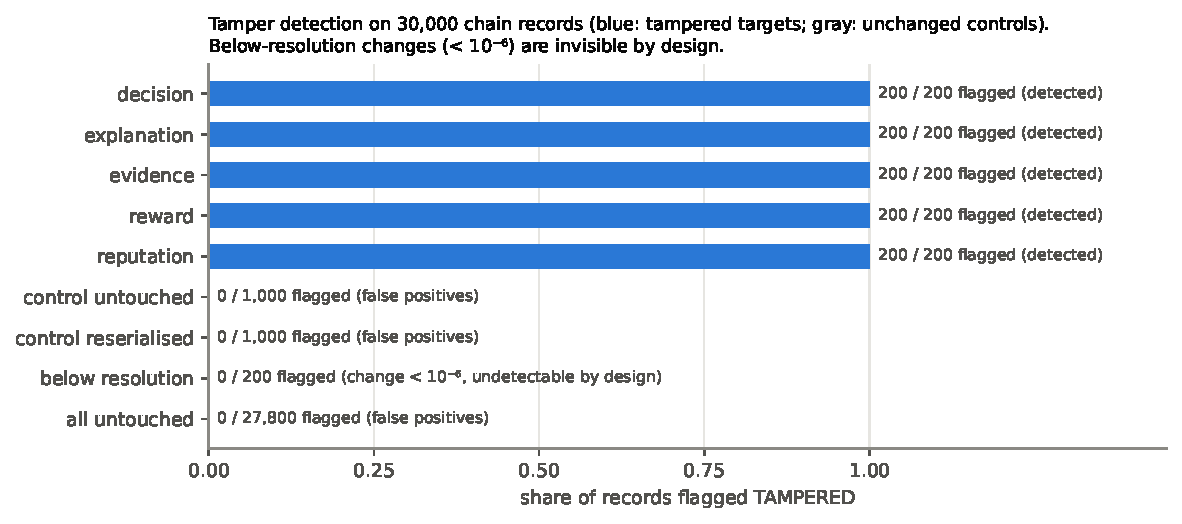
\includegraphics[width=\columnwidth]{figures/fig7_tampering.pdf}
\caption{Share of records flagged as tampered, by target and control group}
\label{fig:tamper}
\end{figure}

The provenance layer recorded 30{,}000 agent-round records from the LLM main runs of both
domains on a local Ethereum-compatible node. Of 1{,}000 records altered off chain, 200 in each
of decision, explanation, evidence, reward and reputation, all were detected; no false
positive occurred in 2{,}000 untouched or re-serialised controls or in the 27{,}800 other
records (Table~\ref{tab:provenance}, Figure~\ref{fig:tamper}). Changes smaller than the
$10^{-6}$ storage resolution of rewards and reputation are invisible by design. The contract
refused all overwrites and writes from another account. In batches of 100, a record cost
about 96{,}000 gas; local-node latency excludes consensus and network delay and will differ
on a production network. H5 is supported in the sense of integrity: the layer shows that
records were not changed, not that they were true.

\begin{table}[t]
\caption{Hardened provenance: agent signatures, model registration and anchoring (amendment 9, descriptive)}\label{tab:hardened}
\footnotesize
\begin{tabular}{@{}ll@{}}
\toprule
Check & Result \\
\midrule
\multicolumn{2}{@{}l}{\emph{Forged or replayed writes (refused by the contract)}} \\
content changed after signing & 0 / 100 accepted \\
signed with another agent's key & 0 / 100 accepted \\
signed with an unregistered key & 0 / 100 accepted \\
replayed under another record id & 0 / 100 accepted \\
replayed from another deployment & 0 / 100 accepted \\
substituted model & 0 / 100 accepted \\
sent by a non-owner account & 0 / 100 accepted \\
correctly signed (control) & 100 / 100 accepted \\
\midrule
\multicolumn{2}{@{}l}{\emph{History rebuilt by the operator}} \\
altered records, amendment-5 check & 0 / 200 detected \\
registrations against anchor & 10 / 10 differ \\
altered records against anchor & 200 / 200 detected \\
unaltered records against anchor & 0 / 29,800 flagged \\
\midrule
\multicolumn{2}{@{}l}{\emph{Honest run}} \\
records, registrations, anchors & 0 tampered, 0 + 0 mismatches \\
\bottomrule
\end{tabular}
\footnotetext{Local nodes, 30,000 records; the anchor chain is a second local node standing in for an external chain. Batches of 100: 126,005 gas per record (amendment 5: 95,912); anchoring 113 gas per record; inclusion proof 320 bytes.}
\end{table}


The hardened variant was tested on the same 30{,}000 records, with the anchor chain simulated
by a second local node (Table~\ref{tab:hardened}). The contract refused every forged or
replayed write: content changed after signing, signatures by another agent's or an
unregistered key, signatures replayed under another record identifier or from another
deployment, and substituted models (100 attempts each), while all 100 correctly signed
control records were accepted. When the operator rebuilt the entire history with 200 altered
records, per-record verification found nothing, as expected when chain and off-chain store
are both replaced; the registrations exposed the operator's keys for all ten agents, and the
anchors identified exactly the 200 altered records, whichever field was changed, with no
unaltered record flagged. The hardening raised the cost to about 126{,}000 gas per record in
batches of 100 (from 96{,}000), plus 113 gas per record for anchoring. These results are
descriptive and rest on the assumption that the anchor chain cannot be rewritten.

\subsection{Cross-domain comparison and sensitivity}\label{sec:cross}

\begin{table*}[t]
\caption{Cross-domain comparison (H6: same verdict in both domains) and robustness of the classical verdicts across $\beta$, $\rho$ and $\omega$}\label{tab:cross}
\footnotesize
\begin{tabular}{@{}lllll@{}}
\toprule
Agents & Outcome & Pharmaceutical & Energy & Same verdict \\
\midrule
Classical & Fidelity $F$ & +83.5\% (improved) & +3.6\% (negligible) & no \\
 & Evidence support $E$ & +75.7\% (improved) & +4.3\% (negligible) & no \\
 & Manipulation $M$ & -69.7\% (improved) & -44.4\% (improved) & yes \\
LLM & Fidelity $F$ & -1.9\% (negligible) & +3.4\% (negligible) & yes \\
 & Evidence support $E$ & -1.0\% (negligible) & -0.3\% (negligible) & yes \\
 & Manipulation $M$ & -22.0\% (improved) & -12.6\% (improved) & yes \\
\midrule
Sensitivity (pharma) & verdicts changed & \multicolumn{3}{l}{none (all values of $\beta$, $\rho$, $\omega$)} \\
Sensitivity (energy) & verdicts changed & \multicolumn{3}{l}{$\omega$: fidelity, evidence} \\
\bottomrule
\end{tabular}
\end{table*}


\begin{figure*}[t]
\centering
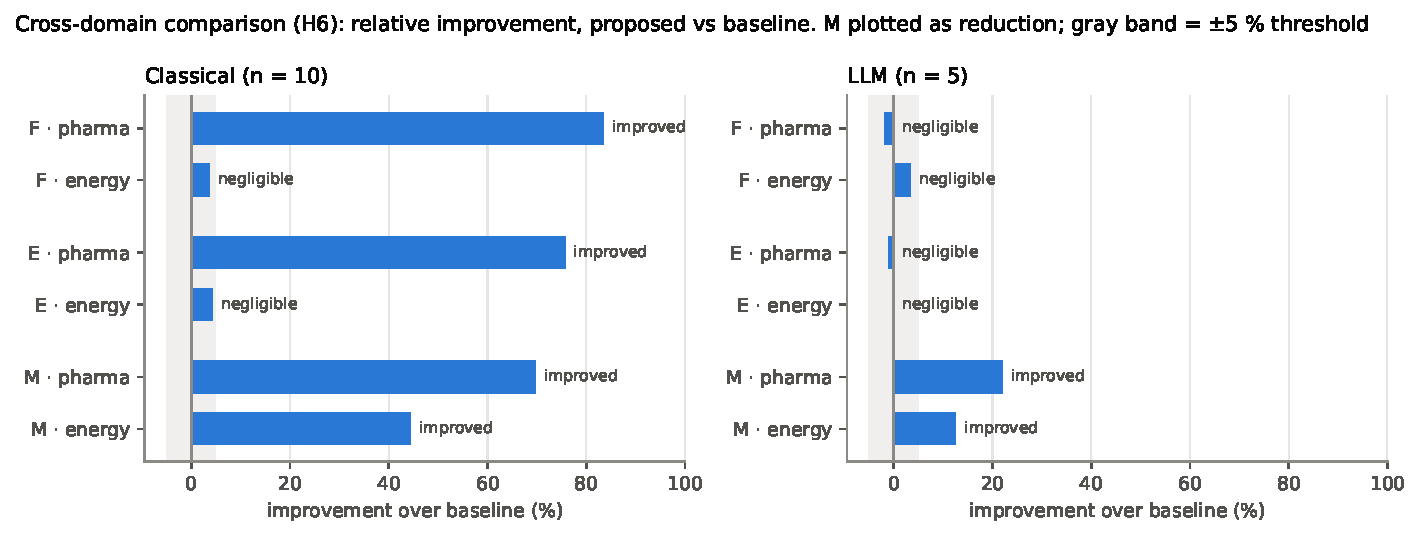
\includegraphics[width=\textwidth]{figures/fig8_cross_domain.pdf}
\caption{Relative improvement of the proposed system over the baseline in each domain;
manipulation is plotted as a reduction; the grey band marks the 5\% threshold}
\label{fig:cross}
\end{figure*}

With classical agents, both domains give the same verdict only for manipulation, so H6 holds
for one of three outcomes (Table~\ref{tab:cross}, Figure~\ref{fig:cross}). The
pharmaceutical verdicts are unchanged at every value of $\beta$, $\rho$ and $\omega$. In
energy they are unchanged across $\beta$ and $\rho$, but fidelity and evidence support change
from negligible to improved at $\omega=0.75$ ($+27.8\%$ and $+28.6\%$): when steering the
decision is worth more, the baseline's explanations deteriorate and the mechanism's
advantage appears. In pharma the fidelity gain persists at $\beta=0$ ($+74.7\%$), so it is
produced by the evidence and manipulation terms together and should not be attributed to the
fidelity weight alone.

\subsection{LLM agents}\label{sec:llmresults}

\begin{table}[t]
\caption{LLM agents: 2$\times$2 wording $\times$ payoff experiment on mean stated confidence ($n=5$ seeds; Holm over the three effects; added after the main analysis)}\label{tab:llm}
\footnotesize
\begin{tabular}{@{}lllll@{}}
\toprule
Domain & Effect & $\Delta$ [95\% CI] & $p$ (Holm) & Verdict \\
\midrule
pharma & wording & -0.299 [-0.306, -0.291] & $<0.0001$ & lower \\
 & payoff & +0.001 [+0.000, +0.002] & 0.0971 & no detectable effect \\
 & interaction & -0.004 [-0.008, -0.000] & 0.0971 & not detected \\
energy & wording & -0.164 [-0.167, -0.161] & $<0.0001$ & lower \\
 & payoff & -0.000 [-0.002, +0.002] & 0.9884 & no detectable effect \\
 & interaction & +0.006 [+0.004, +0.009] & 0.0046 & detected \\
\bottomrule
\end{tabular}
\end{table}


With LLM agents (Table~\ref{tab:cross}), manipulation fell in both domains ($-22.0\%$ and
$-12.6\%$, Holm $p<0.0001$) while fidelity and evidence support were negligible; fidelity
stayed between 0.45 and 0.46 in every system; sample replies show the model misreading the
signs and levels in its own tool output. The fall in manipulation came mostly from lower
stated confidence: the confidence-inflation component accounts for $-0.060$ of the $-0.065$
change in pharma and $-0.029$ of $-0.035$ in energy. To find its
cause we added, after the main analysis, a 2$\times$2 experiment that crosses the wording of
the reward rules in the prompt with the payoff actually applied (Table~\ref{tab:llm}). The
wording lowered confidence by 0.299 in pharma and 0.164 in energy, whereas no payoff effect was
detected in either domain; the energy run, specified before it was carried out, reproduced the
pharmaceutical pattern, with a small wording-by-payoff interaction ($+0.006$) in energy only.
For these agents the behavioural change reflects what they are told, not what they are paid.

%% ---------------------------------------------------------------------------------------
\section{Discussion}\label{sec:discussion}

\paragraph{What the mechanism does.} Putting audited explanation quality into the utility
reliably reduced manipulation: in both domains, with classical and LLM agents, in the ablation
without reputation and across the sensitivity range. It also removed the advantage of false
explanations: in the pharmaceutical case the agents that still deviate do so with truthful
explanations. Whether explanation quality itself improves depends on how much the baseline
leaves to gain. In pharma, where unilateral manipulation pays under a decision-only utility,
the gains were large; in energy, where honesty was already a best response, they were
significant but small, and they became large only when the private stake $\omega$ rose.

\paragraph{What it does not do.} The mechanism did not make the collective decision more
robust to a growing share of agents that always manipulate. It scores reports; it cannot
change the votes of agents that ignore the payoff, and reputation reacts only after several
rounds. Defences against persistent attackers need another instrument, such as exclusion
thresholds or robust aggregation. With LLM agents the improvement cannot be credited to the
payoff: a prompt that states the rules produces the same change. Designers of incentive
mechanisms for LLM agents should therefore test whether agents respond to payoffs at all
before attributing behaviour to them.

\paragraph{Implications.} The results indicate when an explanation-aware incentive is worth
deploying: where agents' private objectives conflict with the collective goal, so that
manipulation pays under a decision-only payoff. There it removes the profit of false
explanations and shifts agents towards truthful reports; where agents are already aligned,
it adds little. It requires an auditor with access to the agents' models, and it has to be
combined with a separate defence for agents that do not respond to incentives at all. For
provenance, designers should state which of integrity, authenticity and truthfulness a
ledger provides; ours provides the first two, and only the audit speaks to the third.

\paragraph{Security scope.} The evaluated threats are dishonest agents with valid identities
(false attribution, inflated confidence, unsupported evidence, strategic voting, collusion of
two), changes to recorded artefacts, and forged, replayed or rewritten records. Out of scope
are attackers who adapt to the utility, Sybil identities and whitewashing (a new identity
starts at reputation 0.5), poisoned source data, models built to mislead SHAP, a declared
model that differs from the one actually run, stolen agent keys, and network-level attacks;
all components ran in one process on one machine. The provenance layer is a research
prototype, not a system hardened against infrastructure attacks.

\paragraph{Limitations.} Both reference decisions are constructed, and decision accuracy means
agreement with them, not with real choices. The pharmaceutical data cover one programme's
antiretroviral and HIV-test deliveries, and the candidate sets are inferred. The energy
battery parameters are simulated. Fidelity is measured against SHAP of the agent's own model
and therefore needs white-box access; it inherits the limits of SHAP and says nothing about
whether the model itself is right. The terciles that define evidence levels and the incentive
weights were set a priori; other choices would give other numbers. Reputation creates path
dependence. Inference rests on ten seeds (five for LLM agents) on one dataset per domain. The
LLM results come from one 7-billion-parameter model, and the factorial experiment was added
after the main analysis, as was the hardened provenance layer, whose anchor chain was simulated
by a second local node. Overhead was measured on local nodes and will differ on production
networks.

%% ---------------------------------------------------------------------------------------
\section{Conclusion}\label{sec:conclusion}

We proposed an explanation-aware incentive for multi-agent AI decisions, in which audited
explanation fidelity, evidence support and manipulation enter each agent's utility,
reputation weights votes and a blockchain records the artefacts, and evaluated it under a
pre-registered protocol on real pharmaceutical and energy data. The incentive reduced
strategic manipulation in both domains and removed the profit of false explanations; it
improved explanation quality strongly only where the baseline left room; it did not increase
robustness to malicious agents; and the provenance layer detected every tampered record and,
with agent signatures and anchoring, refused every forged write and exposed a history rebuilt
by its operator. For
LLM agents, the effect followed the wording of the rules rather than the payoff. Future work
should test the mechanism with black-box fidelity estimates, real decision outcomes, larger
and more diverse LLMs, and defences that act on persistent attackers.

%% ---------------------------------------------------------------------------------------
\backmatter

\section*{Declarations}

\bmhead{Funding} [To be completed on the title page.]

\bmhead{Competing interests} [To be completed on the title page.]

\bmhead{Data availability} The pharmaceutical data are the public USAID SCMS delivery history
\citep{scmsdata2015}; the energy data are available from Mendeley Data
\citep{optirecdata2025}. Processed scenarios are regenerated deterministically by the code.

\bmhead{Code availability} The code, configuration files, frozen protocol with its amendments,
per-experiment summaries and the scripts that generate every table and figure will be released
in a public repository on acceptance; an anonymised copy is available to reviewers.

\bmhead{Author contributions} [To be completed on the title page.]

\bibliography{references}

\end{document}
